\documentclass[spanish]{beamer}
\usetheme{Copenhagen}
\usepackage[utf8]{inputenc}
\usepackage[spanish]{babel}
\usepackage{graphicx}

\title{Oxímetro de pulso}
\author{Gonzalo Vaca}

\begin{document}
\maketitle

\begin{frame}
    \frametitle{Referencias}
    \begin{itemize}
        \item AFE4900 Ultra-low Power, Integrated AFE for Wearable Optical, Electrical Bio-sensing with FIFO. Texas Instruments
        \item STM32LO10F4 Value line ultra-low-power 32-bit MCU Arm-based Cortex-M0+, 16-Kbyte Flash memory, 2-Kbyte SRAM, 128-byte EEPROM, ADC. STMicrolectronics
    \end{itemize}
\end{frame}

\begin{frame}
    \frametitle{Marco normativo}
    \begin{itemize}
        \item Decreto presidencial N° 9763/64 (producción y comercialización de productos médicos)
        \item IEC 60601-2-20 (seguridad eléctrica en equipos médicos)
        \item IEC 62304:2006 (calidad en \emph{software} médico)
        \item ISO 13485:2016 (sistema de gestión de calidad para dispositivos médicos)
        \item Ley 16463/1964 (importación y exportación de productos médicos)
        \item MERCOSUR/GMC/RES N°40/00 (reglamento técnico Mercosur de registro de productos médicos)
        \item Ministerio de Justicia y Derechos Humanos, resolución 41/2001 (Programa Nacional de Garantía de Calidad de la Atención Humana).
    \end{itemize}
\end{frame}

\begin{frame}
    \frametitle{Diagrama en bloques}
    \centering
    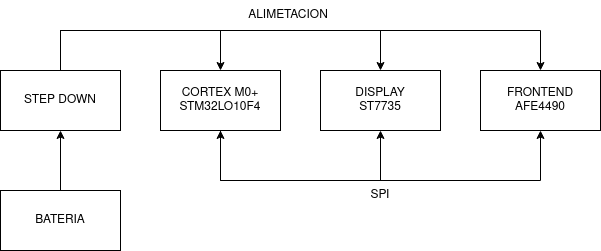
\includegraphics[width=0.8\textwidth]{img/bloques.png}
\end{frame}

\begin{frame}
    \frametitle{Frontend}
    \centering
    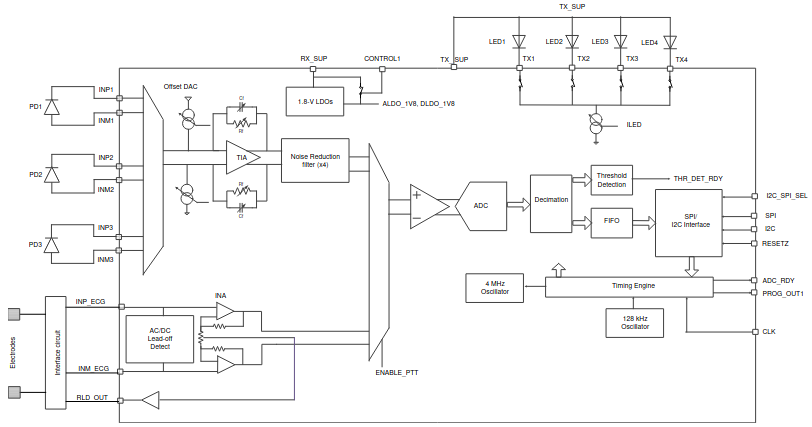
\includegraphics[width=0.8\textwidth]{img/frontend.png}
\end{frame}

\begin{frame}
    \frametitle{Display}
    \centering
    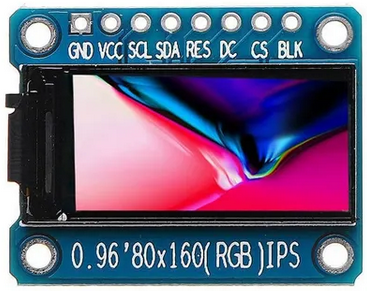
\includegraphics[width=0.8\textwidth]{img/display.png}
\end{frame}

\end{document}
